\chapter{VolPFN and comparative forecasting evidence}
\label{ch:forecast}

We begin the performance evaluation by explaining how VolPFN learns from simulated histories and turns a market history into a forecast. The comparisons then progress from general pretrained forecasters to dedicated financial predictors, realised-risk information and exchange-traded funds. We retain the earlier checkpoint's density evidence separately because it uses a different model. Section~\ref{sec:exposure} records prior contact with every panel. Seed and market breakdowns describe consistency within those evaluations rather than independent significance tests.

\section{Why train on a mixture of volatility processes?}

The turbulent-week illustration in Chapter~\ref{ch:introduction} motivates the simulation design: a persistent shock, a hidden-state change or a new regime can each explain a rise in uncertainty. Training rewards prediction of the next return from the available history \citep{muller2022transformers}. Because stale targets are excluded, the ideal prediction concerns selected positions with the weighting defined in Appendix~\ref{app:technical}. The implemented network approximates that target; whether the learned rule helps on markets remains an empirical question.

Similar observed returns can arise from different simulated processes. We therefore include shock-driven dynamics, hidden states, abrupt switches and lattice shifts in the prior (Table~\ref{tab:simulation-prior}). The mixture exposes training to histories from each of these processes. Including a family does not establish that it is necessary.

\begin{table}[!htbp]
\centering
\caption[Synthetic prior components]{Broad synthetic prior used in the corrected construction. Probabilities are read from \code{volpfn\_prior.py}.}
\label{tab:simulation-prior}
\small
\begin{tabular}{p{0.19\textwidth}rp{0.59\textwidth}}
\toprule
Family & Probability & Main source of variation \\
\midrule
GARCH & 0.20 & Persistent variance recursion with random persistence and innovation response \\
GJR-GARCH & 0.15 & An additional response to negative innovations \\
EGARCH & 0.10 & Log-variance recursion with signed and absolute innovations \\
Stochastic volatility & 0.20 & Persistent latent log variance with optional lagged leverage \\
Rough volatility & 0.10 & Gaussian log variance with Mat\'ern covariance and varying smoothness \\
Markov switching & 0.12 & Two or three variance levels and random expected regime durations \\
Lattice jumps & 0.13 & Reflected jumps between log-variance levels \\
\bottomrule
\end{tabular}
\end{table}

The families vary the source of volatility changes. GARCH, GJR and EGARCH provide persistence and shock responses, with the latter two allowing sign-dependent responses \citep{bollerslev1986generalized,glosten1993relation,nelson1991conditional}. Stochastic volatility adds hidden states \citep{harvey1994multivariate}, while a Mat\'ern construction varies smoothness with motivation from rough volatility \citep{gatheral2018volatility}. This finite Gaussian construction does not cover every continuous-time rough model. Switching and lattice jumps add discontinuities. The listed probabilities distribute training effort; they do not estimate market frequencies.

We also vary the new random shock, termed an \emph{innovation}. Its law is Gaussian with probability 0.25 and otherwise Student with degrees of freedom from 2.5 to 50; a quarter of draws introduce skewness. Standardising to zero mean and unit variance separates innovation shape from volatility level \citep{fernandez1998bayesian}. Independent modifications then add jumps, serial correlation, drift and stale prices with probabilities 0.30, 0.30, 0.50 and 0.25. These remain simulation settings rather than measured frequencies of market behaviour.

Stale prices record zero returns until the accumulated movement is released. Both training losses mask stale next-return targets. Auxiliary labels add jump variance and sum variance over the released interval, but omit possible covariance between successive returns. They therefore supply extra supervision without representing exact conditional risk for every modified process. Return prediction remains the main objective. Both matched designs share these innovations and modifications, leaving the latent-volatility design as the change tested in Chapter~\ref{ch:analysis}.

\section{Why this forecasting representation?}

\begin{figure}[!htbp]
\centering
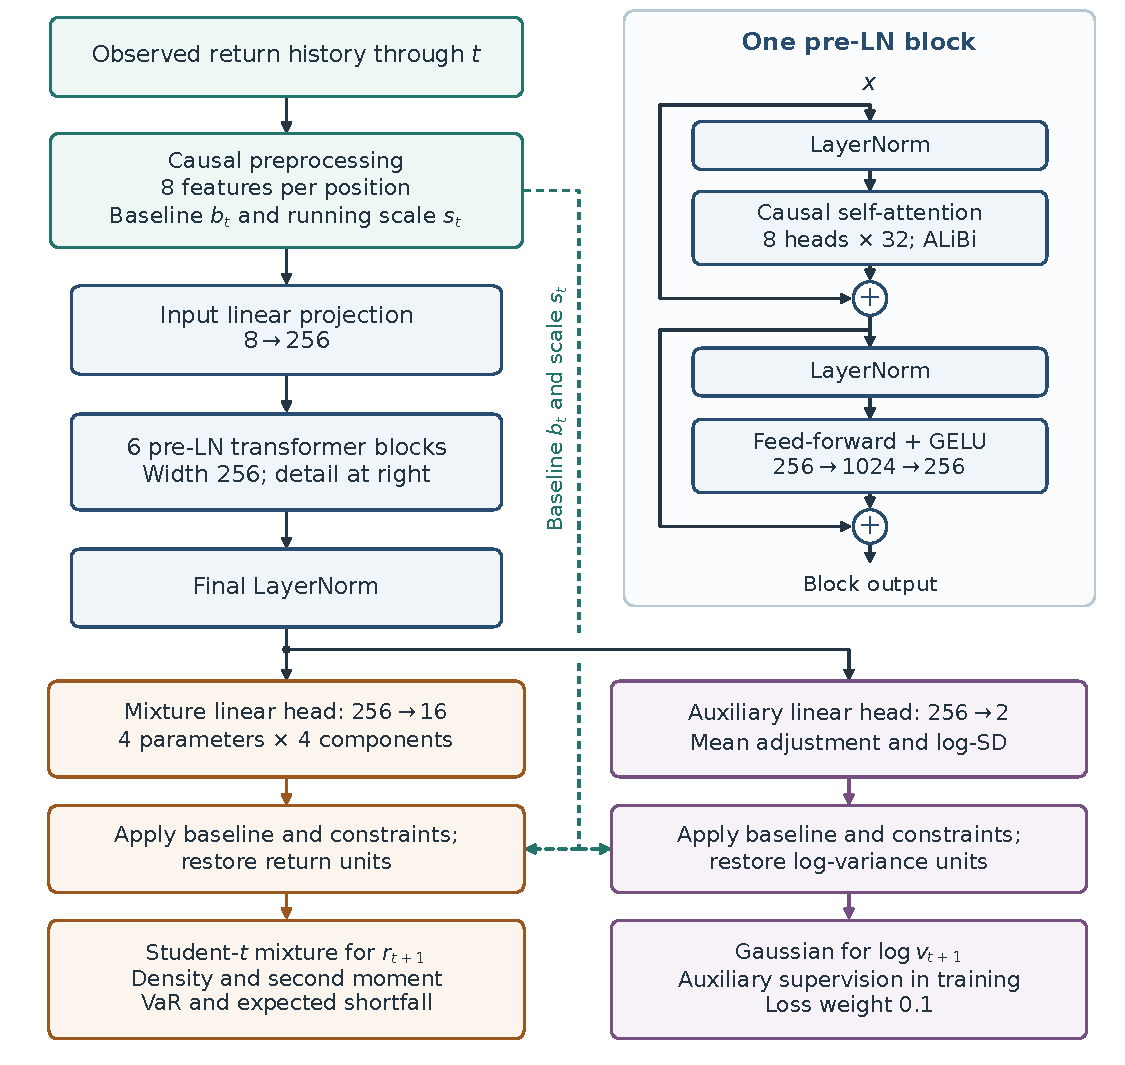
\includegraphics[width=\textwidth]{volpfn_architecture.pdf}
\caption[The implemented VolPFN architecture]{The architecture used by both prior arms. Each input position produces a distribution for the next return. The diagram is drawn from the verified implementation: self-attention and feed-forward components follow \citet{vaswani2017attention}, with pre-normalisation \citep{xiong2020layer} and an ALiBi-based distance bias \citep{press2022alibi}. The baseline uses an exponential average with a half-life of 20 nonzero observations and enters both output transformations. The auxiliary head supplies training supervision; the return forecast comes from the four-component mixture.}
\label{fig:volpfn-architecture}
\end{figure}

The input representation summarises the available history through eight channels: standardised return, magnitude, sign, zero status, three exponential risk estimates and position. Causal attention excludes future returns. The multiple risk horizons help distinguish a recent shock from a sustained change, following earlier volatility-modelling motivation without establishing each horizon as optimal \citep{corsi2009simple}. Appendix~\ref{app:forecast-details} specifies the transformations, layer sizes and distance-bias schedule \citep{vaswani2017attention,xiong2020layer,press2022alibi}.

To turn that representation into a return forecast, we combine four Student components. Their centres, scales and tail thicknesses can differ, giving more flexibility than one fixed Student law \citep{bishop1994mixture}. The issued density is

\begin{equation}
 q_t(x)=\sum_{k=1}^{4}w_{k,t}\,
 \frac{1}{s_{k,t}}f_{\nu_{k,t}}\!\left(\frac{x-\mu_{k,t}}{s_{k,t}}\right),
 \qquad \sum_k w_{k,t}=1.
 \label{eq:volpfn-density}
\end{equation}

The component law $f_\nu$ is the standard Student density; $w$, $\mu$, $s$ and $\nu$ denote weight, centre, scale and degrees of freedom. Weights are non-negative and sum to one, scales are positive, and degrees of freedom exceed two so that second moments exist. The network adjusts an exponential risk baseline that supplies the overall level. This baseline brings a running summary of past squared returns into the output transformation; the component parameters turn that baseline into a complete return distribution. From the mixture we obtain both the density and expected squared return, then subtract squared predictive mean when central variance is required.

Training connects these outputs to two objectives. The main return-density loss rewards probability assigned to observed returns. An auxiliary head predicts simulated log variance and its uncertainty through Gaussian negative log likelihood \citep{caruana1997multitask}, weighted 0.1. Its role is supervision, not the issued risk forecast, and both losses exclude stale targets. Chapter~\ref{ch:analysis} tests removal of the auxiliary objective and direct second-moment prediction. Chapter~\ref{ch:data} gives AdamW and the fixed allocation \citep{loshchilov2019decoupled}.

During market forecasting, new observations change the supplied history and its causal summaries, while the neural weights remain fixed. The forecast can therefore respond to market conditions without further neural training. Future-observation perturbations and input-window ownership checks confirm the causal implementation. We keep evidence from the retained earlier checkpoint separate because its normalisation differs from the corrected procedure.

\section{Corrected comparison with general pretrained forecasters}

\subsection{The comparison that the benchmark answers}

The first benchmark evaluates VolPFN alongside the specified Chronos-2, Moirai-2 and TabPFN-TS adapters \citep{ansari2025chronos2,liu2025moirai2,hoo2025tables}. All score the same 8,774 observations from 28 indices in April 2015--June 2016. Competitor forecasts stay fixed, while each of the five corrected VolPFN models fits a scale adjustment on the same development origins. We then evaluate fixed-calibration squared-return QLIKE with equal market weights and lower loss preferred.

This design ranks complete forecasting procedures. The systems differ in training data, representations and whether their output is a median or mean, so the result cannot isolate the prior's contribution. We address that narrower question through the controlled comparison in Section~\ref{sec:matched-prior}.

\subsection{Magnitude, uncertainty and consistency}

\begin{table}[!htbp]
\centering\small
\caption[Corrected five-model benchmark]{Corrected procedure: competitor minus VolPFN fixed-scale QLIKE. Positive gains favour VolPFN. Family-adjusted intervals and Holm-adjusted $p$-values concern the three primary comparisons with 10-date blocks. The sample is 8,774 market--date rows across 28 markets.}
\label{tab:corrected-benchmark}
\begin{tabular}{lrrrr}
\toprule
Comparator & Gain & Family 95\% interval & Holm $p$ & Markets \\
\midrule
Chronos-2 & 0.08083 & $[0.02265,0.15673]$ & 0.01220 & 26/28 \\
Moirai-2 & 0.07250 & $[0.02327,0.14085]$ & 0.01220 & 26/28 \\
TabPFN-TS & 0.14109 & $[0.07691,0.21846]$ & 0.00015 & 28/28 \\
\bottomrule
\end{tabular}
\end{table}

VolPFN leads the tested calibrated benchmark (Table~\ref{tab:corrected-benchmark}), with QLIKE gains of about 0.081, 0.073 and 0.141 over Chronos-2, Moirai-2 and TabPFN-TS respectively. Every seed improves on every comparator, and all three family intervals are positive. These gains are absolute loss differences rather than accuracy percentages. Market breakdowns retain the exceptions: Chronos-2 and Moirai-2 each win on two markets, while VolPFN improves on TabPFN-TS in all 28. This performance claim is limited to the specified calibrated alternatives.

\begin{figure}[!htbp]
\centering
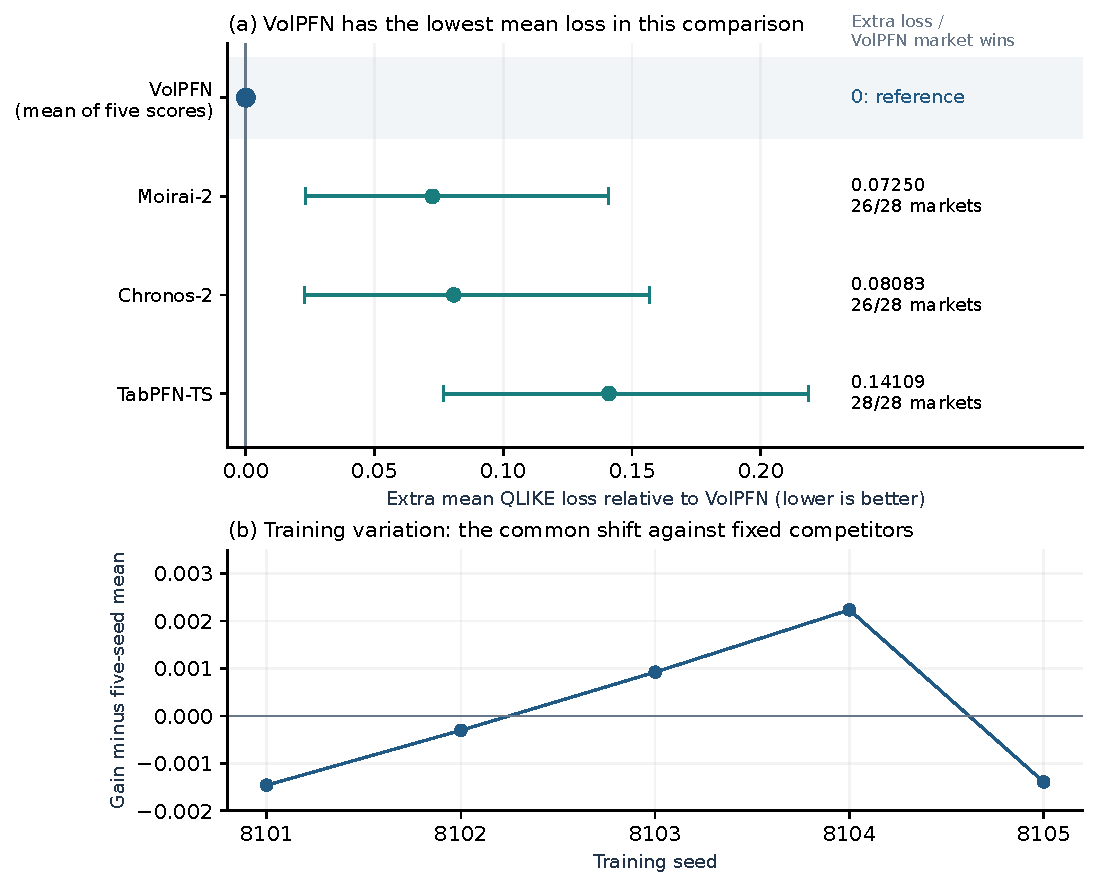
\includegraphics[width=\textwidth]{forecasting_benchmark_rank.pdf}
\caption[VolPFN leads the tested benchmark comparison]{Fixed-scale QLIKE on 8,774 rows across 28 markets, April 2015--June 2016. Top: competitors' excess loss relative to the mean score of five VolPFN models, with family-adjusted 95\% calendar-block intervals and market wins. VolPFN's zero is a reference, not an estimate with zero uncertainty. Bottom: each seed's gain minus the five-model mean; this shift is common across fixed competitors. Scores are averaged across models, not ensemble predictions. The recorded adapters, fitted development scales and historical exposure define the comparison.}
\label{fig:corrected-benchmark}
\end{figure}

All three conclusions survive the alternative calendar-block lengths. Figure~\ref{fig:corrected-benchmark} also shows that similar mean scores across seeds can coexist with appreciable uncertainty across dates. Appendix~\ref{sec:supplementary-forecasting} retains the complete seed and market breakdowns. The supported claim remains performance of these calibrated pipelines on this panel.

\FloatBarrier

\section{Financial benchmarks and realised-risk information}

We next broaden the competitor set and the information supplied to forecasts. Because these studies use different periods and separately adjusted families, each result needs to be interpreted within its own comparison. Table~\ref{tab:study_map} records those boundaries.

\subsection{Dedicated daily financial predictors}
\label{sec:new-daily-comparison}

The completed ARCH-LSTM, GARCH-LSTM and GINN adaptations provide dedicated daily financial comparisons on 28 markets in 2015--February 2022. We compare their squared-return QLIKE with full VolPFN on the retained observations, reporting each competitor's loss minus full's loss. Full improves over all three, with gains of about 0.046--0.376 (Table~\ref{tab:new-daily-gains}). All five seed means and all 28 market means favour it, and block-length sensitivities retain the adjusted conclusions. Full is the pre-specified reference, selected before inspecting these comparison outcomes.

\begin{table}[!htbp]\centering
\begingroup\small\setlength{\tabcolsep}{4pt}
\caption[Gains against daily financial neural predictors]{Full VolPFN versus the dedicated daily adaptations, 2015--February 2022. The four-slot external family retains unavailable RECH at $p=1$. Ordinary 95\% intervals are not simultaneous intervals. Gains favour full when positive.}\label{tab:new-daily-gains}
\begin{tabular}{@{}>{\raggedright\arraybackslash}p{4.1cm}rcr@{}}
\toprule
Comparison & Gain & Ordinary 95\% interval & Holm $p$ \\
\midrule
ARCH-LSTM & 0.376213 & $[0.295777,0.453705]$ & 0.000200 \\
GARCH-LSTM & 0.070375 & $[0.050145,0.089188]$ & 0.000200 \\
GINN & 0.046427 & $[0.031970,0.059823]$ & 0.000200 \\
rech & --- & --- & 1.000000 \\
\bottomrule
\end{tabular}\endgroup\end{table}


The financial predictors fit each market separately and have different contexts and validation choices, whereas VolPFN learns from simulation. The comparison therefore concerns these completed adaptations without isolating architecture or reproducing every published setting. Appendix~\ref{sec:new-research-results} retains the failed historical configuration and unavailable RECH comparison alongside the successful procedures.

\subsection{A harmonised daily-return panel}
\label{sec:new-harmonised-daily}

To assess the wider daily leaderboard on common observations, we align saved raw forecasts on 22,026 market--date keys in 2019--February 2022. VolPFN variants lead the evaluated daily-return-only procedures at both squared-return and realised-kernel QLIKE. The set includes conventional volatility models, dedicated financial networks and general pretrained forecasters such as TabPFN-TS. Full scores about 0.704 and 0.626. The complete two-target rule for full supports improvement over ARCH-LSTM, Chronos-2, GARCH-LSTM, TabPFN-TS and UniVol, but not over GJR-GARCH despite a lower mean. Observed leadership consequently does not establish superiority over every competitor.

Noaux and the earlier VolPFN version have slightly lower means than full, but their descriptive ranks do not inherit its tests. The complete leaderboard retains Moirai's floor-associated losses and EGARCH's extreme forecasts as outcomes of the issued procedures (Appendix~\ref{sec:new-research-results}). The independently fitted compact rule remains a separate historical alternative. TTM's lower diagnostic scores involve intraday information and belong to a different information comparison.

\subsection{Adding realised-risk forecasts}
\label{sec:new-intraday-comparison}

We then add intraday information without retraining the daily network by combining its forecast with Tiny Time Mixers (TTM), which uses past realised kernels. We call this additional predictor a \emph{helper}. For market $m$, date $t$, risk target $p$ and seed $s$, the combination is

\begin{equation}
 \log h_{m,t}^{p,s}=a_t^{p,s}+w_t^{p,s}\log h_{A,m,t}^{p,s}
 +(1-w_t^{p,s})\log h_{B,m,t}^{p,s}.
 \label{eq:new-online-blend}
\end{equation}

Here $A$ is the daily predictor and $B$ is the helper. We fit the intercept $a$ and weight $w$ using earlier completed observations pooled across markets. The intercept adjusts the overall level, while the weight changes the relative contributions and may fall outside $[0,1]$ because it is unconstrained. During the first sixty union dates, we use $a=0$ and $w=0.5$, then update every twenty union dates; a union date occurs in at least one included market. Squared-return fitting uses second moment, whereas realised-kernel fitting uses central variance. Since the two targets are fitted separately, their combinations do not define a single return density.

VolPFN+TTM scores about 0.672 and 0.599 at the two targets, while GNNHAR retains lower descriptive means of about 0.669 and 0.595 (Figure~\ref{fig:new-intraday}). The joint rule supports the combination over standalone full VolPFN, the 26 September version and GJR-GARCH. Comparisons with GNNHAR, QLIKE-HAR, Transfer-XGBoost, raw TTM and GJR+TTM remain unresolved. Passing an adjusted test alone is insufficient when its family interval crosses zero; both requirements must hold.

\begin{figure}[!htbp]\centering
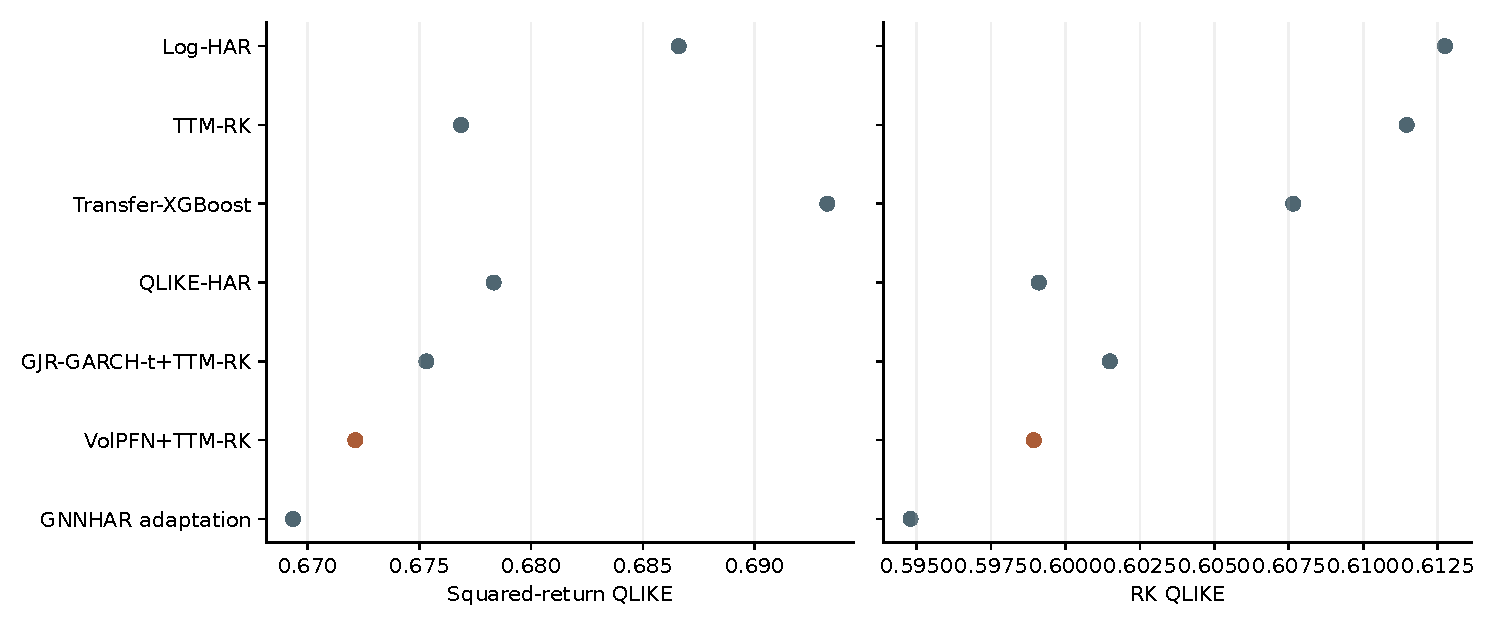
\includegraphics[width=\textwidth]{new_intraday_comparison.pdf}
\caption[Selected realised-risk procedures on common keys]{Descriptive QLIKE for selected complete procedures on the same 2019--February 2022 keys. Both proxy scores retain GNNHAR's lower mean. These points have no significance labels; information access and fitting opportunities differ, and the complete 38-slot rule determines supported comparisons.}
\label{fig:new-intraday}
\end{figure}

The blend changes both the information entering the forecast and the way its level is fitted. To examine the latter explanation, the October follow-up tests whether calibrating TTM alone recovers the combination's advantage on the same 22,026 observations. Its primary control fits $\log h=a+b\log h_{\mathrm{TTM}}$, giving two parameters to adjust level and response, as in the blend. A secondary control fits only a multiplicative scale. Both issue raw TTM during the first sixty union dates, then refit every twenty dates on strictly earlier completed observations pooled across markets. Risk targets are fitted separately. The affine control retains the blend's optimiser and tolerances, and the recorded follow-up replay reproduces its calculation to floating-point precision.

\begin{table}[!htbp]\centering\small
\caption[TTM-only causal calibration controls]{Saved blend and completed TTM-only controls on the same 22,026 keys, 28 markets, 2019--February 2022. Lower QLIKE is better. Raw TTM and GJR+TTM are descriptive here; the four-slot family compares the VolPFN blend with the two calibration controls at both proxies.}
\label{tab:followup-ttm}
\begin{tabular}{lrr}
\toprule
Procedure & Return QLIKE & RK QLIKE \\
\midrule
VolPFN+TTM blend & 0.672139 & 0.598944 \\
GJR+TTM blend & 0.675318 & 0.601493 \\
Saved standalone TTM & 0.676869 & 0.611457 \\
Scale-calibrated TTM & 0.681754 & 0.612566 \\
Affine-calibrated TTM & 0.685450 & 0.622200 \\
\bottomrule\end{tabular}
\end{table}


Control loss minus combination loss measures the gain beyond TTM-only calibration. The affine gains are about 0.013 for squared returns and 0.023 for RK, with adjusted $p=0.002$ and $p=0.004$. Scale-only gains are about 0.010 and 0.014, with adjusted $p=0.004$ and $p<0.001$. Every reference seed improves and all four family intervals are positive; twenty- and 120-date sensitivities retain support (Appendix~\ref{sec:followup-results}). TTM-only calibration worsens its mean score on the saved panel, and a descriptive check excluding the initial period retains the ordering.

The follow-up establishes predictive value beyond those specified calibration controls, without identifying daily information as the unique cause. Warm-up forecasts differ between the controls and blend. Raw TTM and GJR+TTM comparisons remain unresolved, and GNNHAR still has lower descriptive losses. Foreign histories and pooled fitting further restrict attribution to the daily predictor alone. RK publication vintages are also unverified: placing a measurement before the target session does not by itself show that this version of the measurement was available then.

A supplementary XGBoost helper draws 84 features from the target and other markets. All 140 fitted models issued forecasts, and its blend scores about 0.674 and 0.604. However, no contrast passes the separate twelve-comparison joint rule. We have not removed foreign-market inputs with other settings fixed, so their presence does not establish a causal benefit. Appendix~\ref{sec:new-research-results} retains the controls and complete losses.

Additional realised-risk information improves some completed procedures, but the comparisons do not establish this blend as the best realised-risk forecast. This limits the performance claim and separates it from the question of what the standalone daily prior contributes.
\FloatBarrier

\section{Frozen evaluation on a new ETF population}
\label{sec:external-etfs}

The ETF study extends the asset population to test transfer beyond stock-market indices. Original full/noaux weights and the historical model selected on earlier index development data score the same 22,600 session returns from twenty ETFs in March 2022--August 2026. ETF outcomes neither select checkpoints nor update neural weights. Rolling GJR follows the frozen causal fitting policy in Chapter~\ref{ch:data}.

\begin{table}[!htbp]\centering\small
\caption[Frozen external ETF scores]{Frozen twenty-ETF population, 22,600 rows per model/seed, March 2022--August 2026. Means weight ETFs and neural seeds equally. Squared-return QLIKE is primary; native NLL is descriptive. Lower is better. Original full/noaux weights and index-development-selected historical weights receive no ETF training.}
\label{tab:followup-etfs}
\begin{tabular}{lrr}
\toprule
Procedure & Return QLIKE & Native NLL \\
\midrule
Synthetic noaux & 0.437251 & 1.111585 \\
Synthetic full & 0.438591 & 1.111583 \\
Rolling GJR-GARCH-$t$ & 0.452051 & 1.117771 \\
Development-selected historical & 0.458122 & 1.138492 \\
\bottomrule\end{tabular}
\end{table}


On matched ETF observations, noaux improves on the historical procedure by about 0.021 QLIKE units, with Holm-adjusted $p=0.03$ and a positive family interval. All five seed gains and eighteen of twenty ETF means favour noaux, and both alternative block lengths retain support. Full and noaux have lower means than rolling GJR by about 0.013 and 0.015, but adjusted $p$-values near 0.10 and family intervals crossing zero leave superiority unresolved (Appendix~\ref{sec:followup-results}). Native density losses remain descriptive rather than an additional superiority endpoint.

This supports the synthetic procedure over the improved historical comparator on the fixed external population. It does not repeat broad--Mat\'ern matching: training source, regularisation and checkpoint selection differ. The protocol predates acquisition, while human exposure remains unverified and the dates share index-study shocks. We therefore interpret this as external population validation subject to those qualifications. The following density results use an earlier checkpoint and another fitting schedule, so their margins stay separate.
\FloatBarrier

\section{Historical density comparisons}
\label{sec:historical-density}

The retained earlier checkpoint allows us to evaluate complete return distributions alongside risk forecasts. It differs from the corrected five-model set and uses repaired causal inference on 28 indices: 26,293 development observations in 2011--2014 and 50,073 later observations in 2015--February 2022. These results complement, rather than replace, the corrected comparisons.

We compare its densities with rolling GARCH-$t$, UniVol and EWMA$(0.94)$ with $t_8$ tails \citep{bollerslev1986generalized,riskmetrics1996}. GARCH fits 1,000 preceding returns every 250 observations. UniVol combines score-driven filters and restart experts, updating their weights through log score. Appendix~\ref{sec:supplementary-forecasting} preserves the schedules and expert grid.

\subsection{What native and common-law scores reveal}

Native scoring evaluates each complete issued distribution, allowing both its scale and shape to affect the result. Common-$t_8$ scoring instead compares scale under one Student law: GARCH supplies variance with fitted mean suppressed, while VolPFN and UniVol supply second moments. UniVol uses its mixture's arithmetic moment rather than its geometric point forecast. All three forecasts are scored under the common law, while the other procedural differences remain.

\begin{table}[!htbp]
\centering
\caption[Development density comparisons]{Development log-density differences, 2011--2014. Positive values favour VolPFN. Intervals are conditional circular observed-date bootstrap intervals.}
\label{tab:development-density}
\small
\begin{tabular}{llrrr}
\toprule
Comparator & Distribution & Difference & 95\% interval & Markets \\
\midrule
GARCH-$t$ & Native & $+0.01714$ & $[0.01352,0.02102]$ & 28/28 \\
UniVol & Native & $+0.01211$ & $[0.00751,0.01662]$ & 27/28 \\
GARCH & Common $t_8$ & $+0.01327$ & $[0.00951,0.01739]$ & 26/28 \\
UniVol & Common $t_8$ & $+0.01025$ & $[0.00665,0.01385]$ & 27/28 \\
\bottomrule
\end{tabular}
\end{table}

Positive development gains under the common law show that flexible shape cannot account for the whole native-density advantage (Table~\ref{tab:development-density}). Subtracting the two margins would not isolate shape because both forecasts change. We instead exchange saved scales and standardised shapes in both replacement orders and average their contributions. The substitution assigns about 0.0078 nats to scale and 0.0043 to shape (Table~\ref{tab:clarity-precision}), with shape including centres, asymmetry and mixture structure. It describes differences between issued forecasts rather than causes in training.

\begin{figure}[!htbp]
\centering
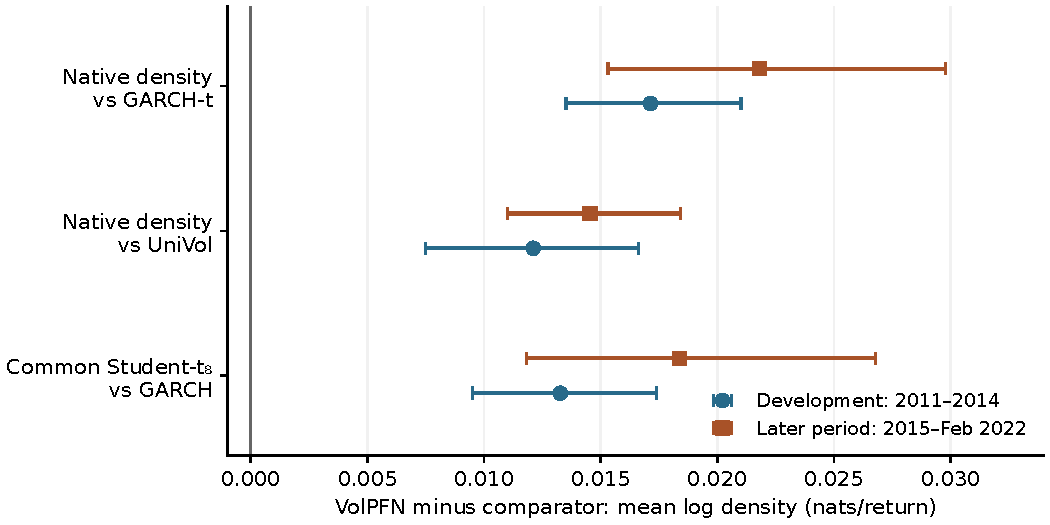
\includegraphics[width=\textwidth]{density_comparison_new.pdf}
\caption[Density gains in two evaluation periods]{Retained-checkpoint equal-market log-density differences on 28 indices. Bars show 95\% circular observed-date bootstrap intervals, conditional on the retained forecasts. Positive values favour VolPFN. They exclude training and model-selection uncertainty; the later period has the prior exposure described in the text.}
\label{fig:density-new}
\end{figure}

The historical later-period rule requires a positive panel mean, bootstrap tail area below 0.05 and gains in at least twenty of 28 markets. We measure calendar uncertainty through 2,000 circular resamples of sixty observed union dates, moving markets together to retain shared shocks. This rule is distinct from the corrected benchmark's multiplicity adjustment.

\begin{table}[!htbp]
\centering
\caption[Later-period density comparisons]{Later-period density comparison, 2015--February 2022. Differences are in nats per return and give equal weight to each of 28 markets.}
\label{tab:confirmation-density}
\small
\begin{tabular}{llrrr}
\toprule
Comparator & Distribution & Difference & 95\% interval & Markets \\
\midrule
GARCH-$t$ & Native & $+0.02181$ & $[0.01532,0.02977]$ & 28/28 \\
UniVol & Native & $+0.01454$ & $[0.01102,0.01841]$ & 28/28 \\
EWMA$(0.94)$--$t_8$ & Native & $+0.02453$ & $[0.01833,0.03169]$ & 28/28 \\
GARCH & Common $t_8$ & $+0.01838$ & $[0.01182,0.02677]$ & 28/28 \\
\bottomrule
\end{tabular}
\end{table}

All four retained later-period comparisons satisfy the historical rule and favour VolPFN in all 28 markets (Table~\ref{tab:confirmation-density}). Native gains are about 0.015--0.025 nats per return, and the common-law GARCH gain is positive. Archived two-sided tail areas reach the resampling floor. These comparisons meet the historical decision rule; they are outside the corrected benchmark family.

The intervals describe date variation conditional on retained forecasts. Prior contact with the pipeline and tail data, documented in Section~\ref{sec:exposure}, restricts their interpretation as independent confirmation.

Market and yearly breakdowns show variation in the margin without identifying one shared crisis mechanism (Appendix~\ref{sec:supplementary-forecasting}). Appendix~\ref{app:alternative-checks} retains the supporting density-average and finite-prior comparisons.

VolPFN's lead in the tested general benchmark and its variants' lead in the daily-return-only leaderboard leave two questions open: how much the prior contributes and how much performance a simpler rule can retain. The next chapter examines both by matching neural training settings and fitting compact rules. Superiority over the stronger realised-risk alternatives remains unresolved.
